\section{Marco teórico}

\subsection{Convexidad}

El concepto de convexidad en los problemas de optimización es de gran importancia. Este concepto aporta una mayor facilidad al resolver un problema. La convexidad puede ser aplicado a conjunto o funciones. Se dice que $S$ es un conjunto convexo si un segmento de linea conecta cualquier par de puntos en $S$. Sean $x,y \in S$, entonces $\alpha x + (1-\alpha)y \in S$ donde $\alpha \in [0,1]$. Se dice que una función es convexa si su dominio $S$ es convexo y cumplen con la propiedad escrita en la ecuación \ref{eq:f_convex}.

\begin{equation}
    f(\alpha x + (1-\alpha)y) \leq \alpha f(x) + (1-\alpha)f(y)
    \label{eq:f_convex}
\end{equation}

Donde $x,y \in S$ y $\alpha \in  [0,1]$.

\subsection{Condiciones necesarias}

Suponiendo que $f: \Real^n \rightarrow \Real$ y que es continuamente diferenciable y $p \in  \Real^n$. Entonces, tenemos que

\begin{equation*}
    f(x+p) = f(x) + \nabla f(x+tp)^T p
\end{equation*}

donde $t\in (0,1)$. De igual manera, si $f$ es doblemente continua diferenciable, entonces se tiene que:

\begin{equation*}
    \nabla f(x+p) = \nabla f(x) \int_0^1 \nabla^2 f(x+tp)p dt
\end{equation*}

por lo tanto

\begin{equation*}
    f(x+p) = f(x)+\nabla f(x)^T p + \frac{1}{2}p^T \nabla f(x+tp) p
\end{equation*}

Con estas hechos, se puede demostrar que si $x^*$ es un punto estacionario entonces el gradiente y el hessiano de $f$ tiene las caracteristicas mostradas en la ecuación \ref{eq:hess_grad_function}.

\begin{equation}
    \nabla f(x^*) = 0 \qquad \nabla^2 f(x^*) \succ 0 \label{eq:hess_grad_function}
\end{equation}

También se puede demostrar que si $\nabla^2 f$ es continua en una vecindad alrededor de $x^*$ y que $\nabla f(x^*)=0$ y $\nabla^2 f(x^*)$ es positiva definida. Entonces $x^*$ es un mínimo local de $f$.

\subsection{Direcciones de búsqueda}

La dirección mas eficiente usando un método de descenso es usar una dirección p descrita en la ecuación \ref{eq:direccion_pk} en cada paso.

\begin{equation}
    p_k = - \nabla f_k \label{eq:direccion_pk}
\end{equation}

En cada iteración de la linea de búsqueda se implementa un cambio en la posición siguiendo la ecuación \ref{eq:direction}.

\begin{equation}
    x_{k+1} = x_{k} + \alpha_k p_k \label{eq:direction}
\end{equation}

Donde $\alpha_k$ es un escalar positivo llamado tamaño de paso.


\subsection{Condiciones de Wolfe \label{sec:wolfe}}

Existen maneras de verificar si el $\alpha_k$ elegido para el k-esimo paso es el óptimo para seguir en la dirección $p_k$. La condición de decrecimiento suficiente esta descrita en la ecuación \ref{eq:armijo_condition}.

\begin{equation}
    f(x_k+\alpha_kp_k) \leq f(x_k)c_1 \alpha_k \nabla f_k^T p_k \label{eq:armijo_condition}
\end{equation}

La interpretación de este resultado es que la función $f$ debe ser proporcional al tamaño de paso $\alpha_k$ y la derivada direccional $\nabla f_k^T p_k$ para una constante $c_1 \in (0,1)$. Esta condición también es conocida como la condición de Armijo.

La condición de decrecimiento suficiente no es la única que se tiene que contemplar, esto debido a que existen $\alpha_k$ muy pequeñas que satisfacen a la desigualdad. Es por ello que se tiene que contemplar la condición de curvatura. La condición de curvatuva esta definida en la ecuación \ref{eq:curvature_condition}.

\begin{equation}
    \nabla f(x_k + \alpha_k p_k)^T  \geq c_2 \nabla f_k^T p_k  \label{eq:curvature_condition}
\end{equation}

Donde $c_2 \in (0,1)$.


La búsqueda de un $\alpha_k$ que cumpla las condiciones de las ecuaciones \ref{eq:armijo_condition} y \ref{eq:curvature_condition} esta descrito en el algoritmo \ref{alg:alpha_algorithm}.

\begin{algorithm}
    \caption{Búsqueda de un $\alpha$ que cumpla las condiciones de las ecuaciones \ref{eq:armijo_condition} y \ref{eq:curvature_condition} \label{alg:alpha_algorithm}}
    $\alpha_0 \gets 0 \qquad \alpha_i \gets 1 \qquad \beta \gets \infty$\\
    \Repeat{
        \If{armijo conditon($\alpha_i$) or curvature contidion($\alpha_i$)}{
            \If{armijo condition($\alpha_i$)}{
                $\beta \gets \alpha_i$\\
                $\alpha_i = \frac{\beta+\alpha}{2}$\\
                \ElseIf{curvature condition ($\alpha_i$)}{
                    $\alpha \gets \alpha_i$ \\
                    \If{$\beta \text{ equals } \infty$}{
                        $\alpha_i \gets 2\alpha$\\
                        \Else{
                            $\alpha_i = \frac{\beta+\alpha}{2}$\\
                        }
                    }
                }
            }
        }
        \Else{break}
    }
    \Return{$\alpha_i$}
\end{algorithm}

\subsection{MNIST}

El conjunto de datos MNIST consta de 70,000 números escritos a mano. Este conjunto de datos fue dividido en datos de entrenamiento (50,000), datos de prueba (10,000) y datos de validación (10,000). Cada imagen esta constitiuda de 28x28 pixeles. En la figura \ref{fig:mnist} se muestran algunos de ellos.

\begin{figure}[H]
    \centering
    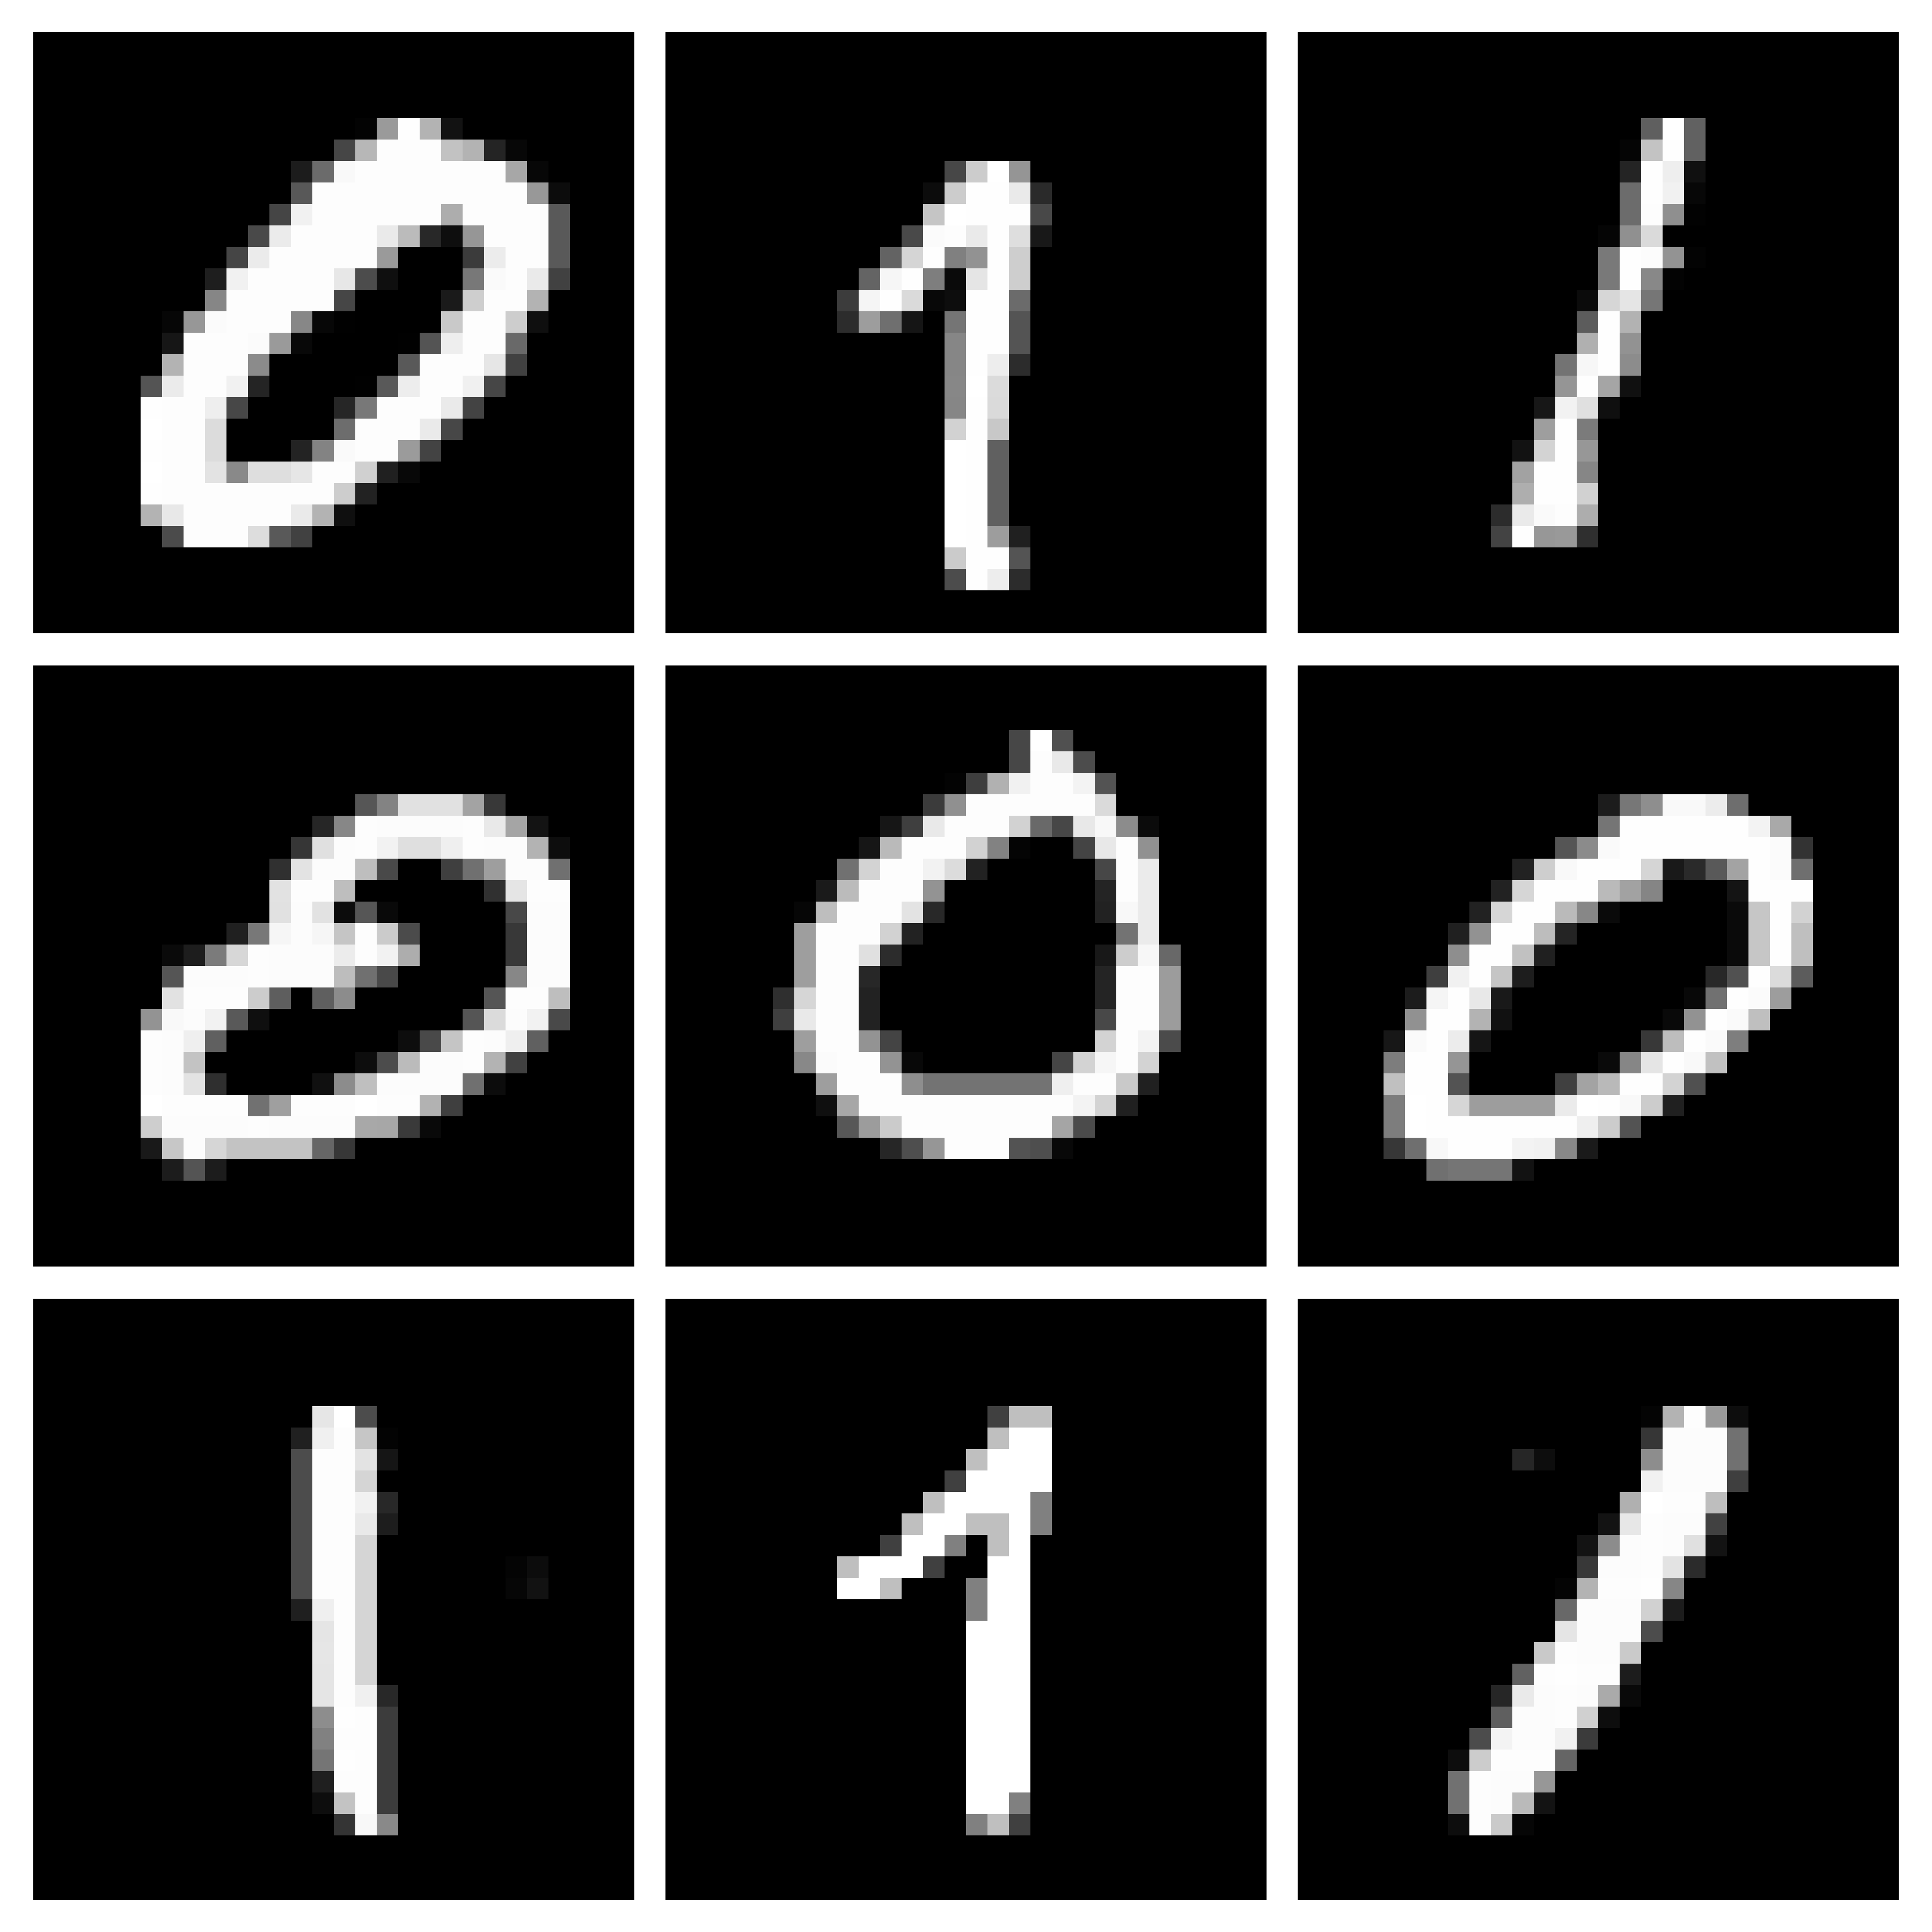
\includegraphics[width=5cm]{Graphics/mnist.png}
    \caption{Algunas imagenes contenidas en el conjunto MNIST.}
    \label{fig:mnist}
\end{figure}

\subsection{Función Log likelihood}

Definimos como la función log likelihood en la ecuación \ref{eq:log_likelihood}.

\begin{equation}
    h(\beta,\beta_0) = \sum_{i=1}^n y_i \log (\pi_i) +(1-y_i) \log (1-\pi_i) \qquad \pi_i(\beta,\beta_0) =  \frac{1}{1+exp(-x_i^T\beta -\beta_0)} \label{eq:log_likelihood}
\end{equation}

donde $x_i \in \Real^n$ y $y_i \in \{0,1,\dots,9\}$. En nuestro caso $n=784$ y $y \in \{0,1\}$. Para obtener una reducción de parametros en la ecuación \ref{eq:log_likelihood} aplicaremos un aumento de dimensión al vector x de tal forma que

\begin{equation*}
    x = [x_0,x_1,\dots,x_{784},1]^T
\end{equation*}

Entonces

\begin{equation*}
    x^T\beta -\beta_0 \rightarrow x^T\beta
\end{equation*}

donde

\begin{equation*}
    \beta = [\beta_1,\beta_2,\dots,\beta_{785},\beta_0]^T
\end{equation*}

por lo que el vector $x$ es ahora elemento del conjunto $\Real^{785}$. Entonces la ecuación \ref{eq:log_likelihood} puede escribirse como en la ecuación .

\begin{equation}
    h(\beta) = \sum_{i=1}^n y_i \log (\pi_i) +(1-y_i) \log (1-\pi_i) \qquad \pi_i(\beta) =  \frac{1}{1+exp(-x_i^T\beta)} \label{eq:log_likelihood_2}
\end{equation}


Calculando el gradiente de la función con respecto a $\beta$ se obtiene lo siguiente:

\begin{align*}
    \dpartial{h}{\beta_j} = \sum_{i=1}^n \frac{y_i}{\pi_i} \dpartial{\pi_i}{\beta_j} + \frac{1-y_i}{1-\pi_i} \dpartial{\pi_i}{\beta_j}
\end{align*}

calculando $\dpartial{\pi_i}{\beta_j}$ se obtiene lo siguiente:

\begin{align*}
    \dpartial{\pi_i}{\beta_j} & = \frac{x_j exp(-x^T_i\beta)}{(1+exp(-x_i^T\beta))^2} \\
                              & = x_j exp(-x_i^T\beta) \pi_i^2                        \\
                              & = x_j (1-\pi_i) \pi_i
\end{align*}

entonces

\begin{align*}
    \dpartial{h}{\beta_j} & =\sum_{i=1}^n \frac{y_i}{\pi_i} \dpartial{\pi_i}{\beta_j} + \frac{1-y_i}{1-\pi_i} \dpartial{\pi_i}{\beta_j} \\
                          & =\sum_{i=1}^n \frac{y_i}{\pi_i} (x_j (1-\pi_i) \pi_i) + \frac{1-y_i}{1-\pi_i} (x_j (1-\pi_i) \pi_i)         \\
                          & =\sum_{i=1}^n x_j y_i(1-\pi_i) - x_j (1-y_i)\pi_i                                                           \\
                          & = \sum_{i=1}^n x_j (y_i-\pi_iy_i+\pi_iy_i-\pi_i)                                                            \\
    \dpartial{h}{\beta_j} & = \sum_{i=1}^n x_j (y_i-\pi_i)
\end{align*}

por lo tanto

\begin{equation}
    \dpartial{h}{\beta_j}  = \sum_{i=1}^n x_j (y_i-\pi_i)   \label{eq:grad_log_likelihood}
\end{equation}

Con su función y gradientes definidos podemos llegar a aplicar el método de descenso de gradiente con una busqueda lineal empleando el algoritmo \ref{alg:alpha_algorithm}.

